
\documentclass[12pt]{article}\usepackage{amsmath}
\usepackage{graphicx}
\usepackage{fancyhdr}
\usepackage{lastpage}
\pagestyle{fancy}
\lhead{\footnotesize \parbox{11cm}{Joel Anna} }
%\lfoot{\footnotesize \parbox{11cm}{\textit{2}}}
\cfoot{}
\rhead{\footnotesize HW2:  \thepage\ of \pageref{LastPage}}
%\rfoot{\footnotesize Page \thepage\ of \pageref{LastPage}}
\renewcommand{\headheight}{24pt}
%\renewcommand{\footrulewidth}{0.4pt}

\begin{document}
\author{Joel Anna<annajoel@pdx.edu>}
\noindent
\underline{Question 1:}\\
To make a perceptually uniform intensity system with intensities
$l_1 = 1, l_2, l_3, l_4, l_5 = 256$:\\
$l_2 = 4, l_3 = 16, l_4 = 64$
\\\\
\underline{Question 2:}\\
a.
\begin{tabular}{|ccc|ccc|ccc|}
\hline
&RGB& & &XYZ& & &L*a*b*&\\
\hline
(0.5,&0,&0) & (0.2062,& 0.1063,& 0.00965) & (38.95,& 63.59,& 53.35)\\
(1,&1,& 1) & (0.9505,& 0.9998,& 1.089) & (99.99,& 0.04123,& -0.02846)\\
\hline
\end{tabular}\\
b.
\begin{tabular}{|c|ccc|}
\hline
u & &RGB& \\
\hline
0 & (0.5,&0,&0) \\
\hline
0.25 & (0.625,&0.25,& 0.25) \\
\hline
0.5 & (0.75,&0.5,& 0.5) \\
\hline
0.75 & (0.875,&0.75,& 0.75) \\
\hline
1 & (1,&1,& 1) \\
\hline
\end{tabular}\\
c.
\begin{tabular}{|c|ccc|ccc|ccc|}
\hline
u &  &XYZ& & &L*a*b*&\\
\hline
0  & (0.2062,& 0.1063,& 0.00965) & (38.95,& 63.59,& 53.35)\\
\hline
0.25  & (0.3923,& 0.3297,& 0.2795) & (64.13,& 26.86,& 11.05) \\
\hline
0.5  & (0.5784,& 0.5531,& 0.5493) & (79.22,& 13.28,& 4.947)  \\
\hline
0.75 & (0.7644,& 0.7764&, 0.8192) & (90.62,& 5.430,& 1.917)\\
\hline
1  & (0.9505,& 0.9998,& 1.089) & (99.99,& 0.04123,& -0.02846)\\
\hline
\end{tabular}
\pagebreak\\
d.\\
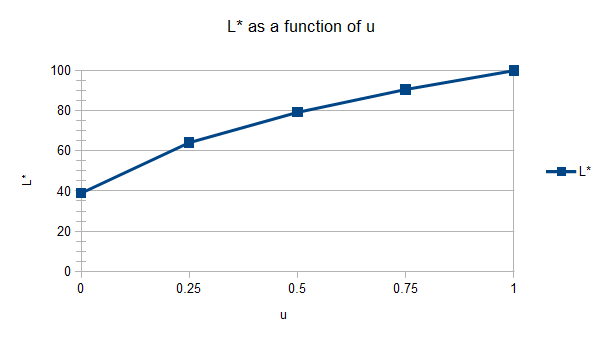
\includegraphics[scale=1]{a.png}
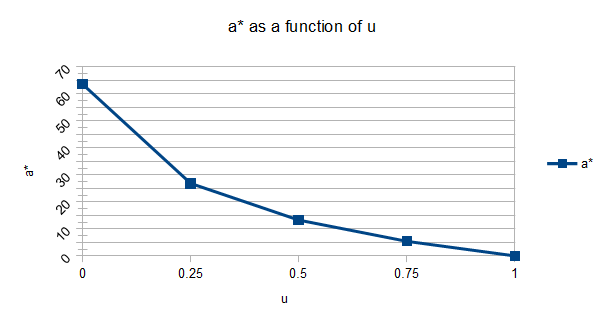
\includegraphics[scale=1]{b.png}
\pagebreak\\
\underline{Question 3:}\\
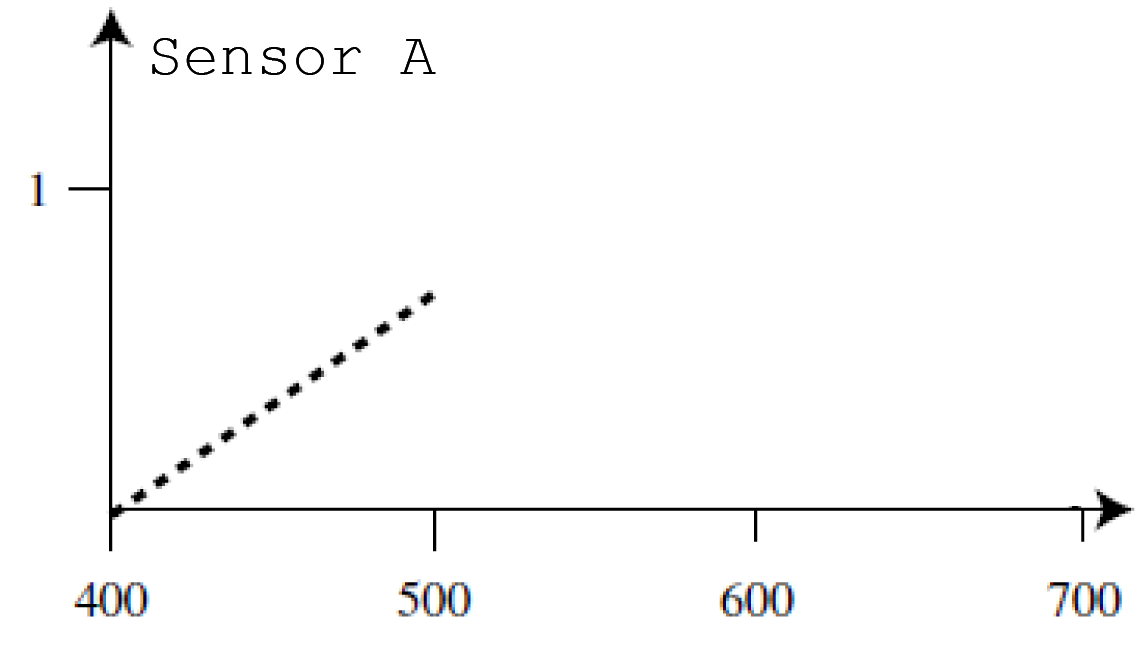
\includegraphics[scale=1]{SensorA.png}\\
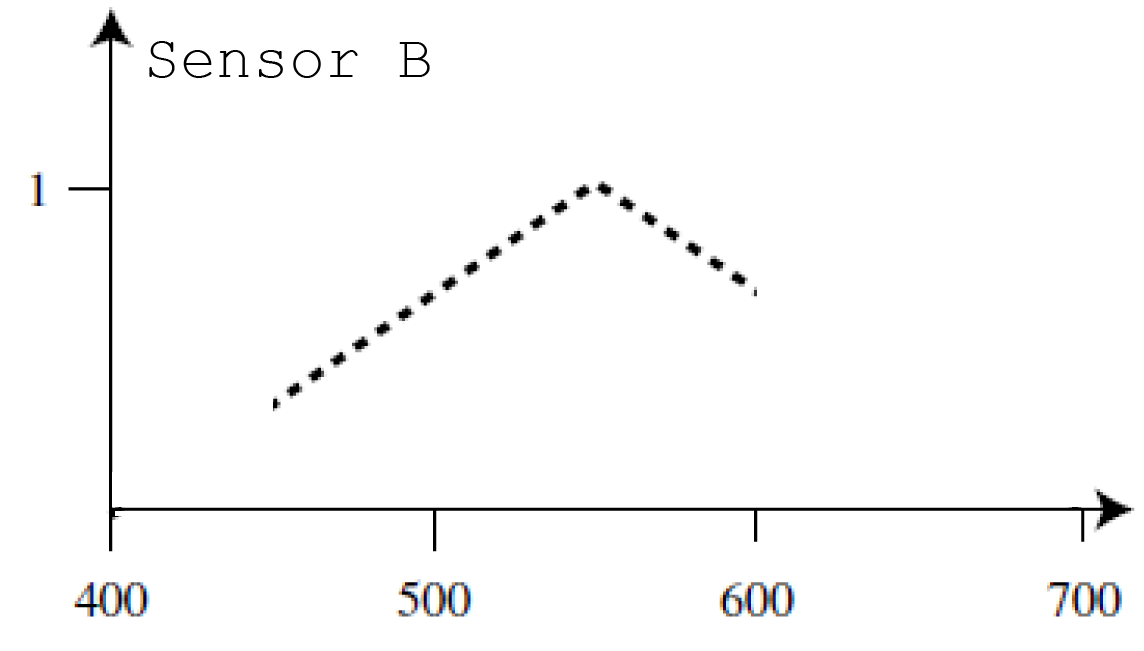
\includegraphics[scale=1]{SensorB.png}\\
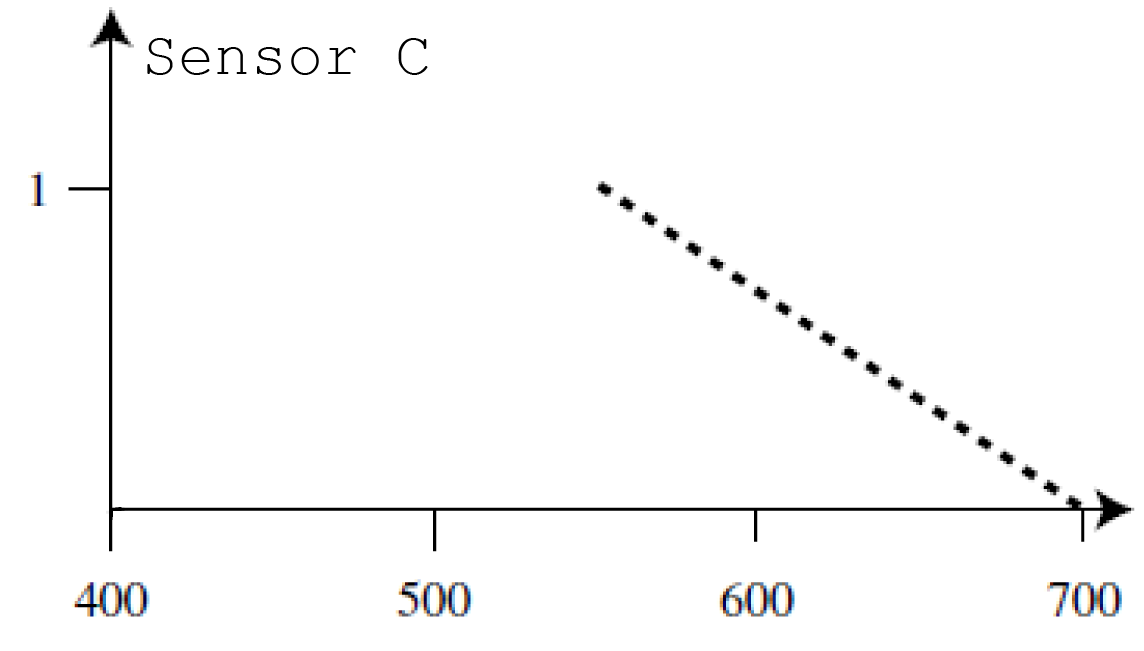
\includegraphics[scale=1]{SensorC.png}\\
\pagebreak\\
\underline{Question 4:}\\
a.
$\begin{bmatrix}
\;\; 0&\;\; 0&\;\; 0&\;\; 0\\
-4&-4&-4&-4\\
-4&-4&-4&-4\\
 \;\;0&\;\; 0&\;\; 0&\;\; 0\\
\end{bmatrix}$
b.
$\begin{bmatrix}
\;\; 0&\;\; 0&\;\; 0&\;\; 0\\
\;\; 0&\;\; 0&\;\; 0&\;\; 0\\
\;\; 0&\;\; 0&\;\; 0&\;\; 0\\
 \;\;0&\;\; 0&\;\; 0&\;\; 0\\
\end{bmatrix}$
c.
$\begin{bmatrix}
1 & 0 & -1\\
2 & 0 & -2\\
1 & 0 & -1
\end{bmatrix}$
\\\\
\underline{Question 5:}\\
1d filter mask = [$a_0,\; a_1,\; ...,\;a_{i-1}$] s.t. $a_j = C^{i-1}_j$\\
1d filtermask for 9:\\
m = $[ 1, 8, 28, 56, 70, 56, 28, 8, 1]$\\
9x9 filtermask: = $M_{ij} = $m$[i] * $m$[j]$\\\\
$\begin{bmatrix}
1&8&28&56&70&56&28&8&1\\
8&64&224&448&560&448&224&64&8\\
28&224&784&1568&1960&1568&784&224&28\\
56&448&1568&3136&3920&3136&1568&448&56\\
70&560&1960&3920&4900&3920&1960&560&70\\
56&448&1568&3136&3920&3136&1568&448&56\\
28&224&784&1568&1960&1568&784&224&28\\
8&64&224&448&560&448&224&64&8\\
1&8&28&56&70&56&28&8&1\\
\end{bmatrix}$



\end{document}

